\documentclass[12pt]{report}

% Code
\usepackage{color}
\usepackage{listing-js}
\lstset{style=boxed}

% Template
\usepackage[utf8]{inputenc}
\usepackage[a4paper]{geometry}
\usepackage[myheadings]{fullpage}
\usepackage{fancyhdr}
\usepackage{lastpage}
\usepackage{graphicx, wrapfig, subcaption, setspace, booktabs}
\usepackage[T1]{fontenc}
\usepackage[font=small, labelfont=bf]{caption}
\usepackage{fourier}
\usepackage[protrusion=true, expansion=true]{microtype}
\usepackage[english]{babel}
\usepackage{sectsty}
\usepackage{url, lipsum}
\usepackage{tgbonum}
\usepackage{hyperref}
\usepackage{xcolor}

\pagestyle{fancy}
%\renewcommand\headrulewidth{0pt}
\cfoot{\thepage}

\newcommand{\HRule}[1]{\rule{\linewidth}{#1}}
\onehalfspacing
\setcounter{tocdepth}{1}

% Format chapter and section
\usepackage{titlesec}
\titleformat{\chapter}{\normalfont\bfseries}{\huge\thechapter}{1em}{\Huge}
\titleformat{\section}{\normalfont\bfseries}{\large\thesection}{1em}{\Large}
\titlespacing*{\chapter}{0pt}{10pt}{40pt}

\begin{document}
\fontfamily{cmr}\selectfont
%\titlehead{\centering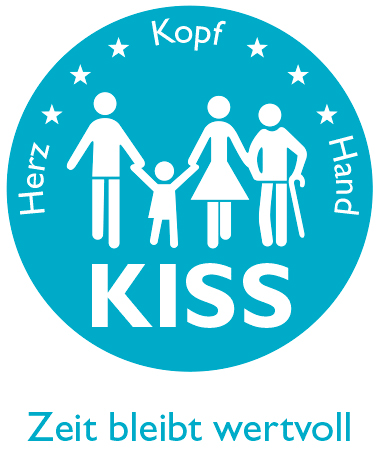
\includegraphics[width=4cm]{kiss.png}}
\title{
\vspace{-40mm}
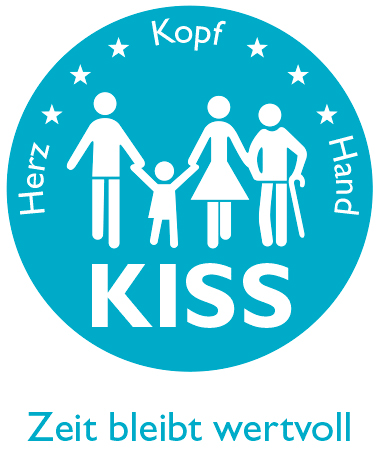
\includegraphics[width=6cm]{kiss.png}
\normalsize \textsc{}
		\HRule{0.5pt}
		\LARGE \textbf{bETHerCare
		\HRule{2pt} \\ [0.5cm]
		\normalsize }
}
\author{
\small Nicolas Aymon \texttt{(naymon@student.ethz.ch}),
\small Alexandru Dan \texttt{(aledan@student.ethz.ch)},\\
\small Betim Djambazi \texttt{(betimd@student.ethz.ch)},
 Johannes Gasser \texttt{(jgasser@student.ethz.ch)},\\
\small Yves Haberth{\"u}r \texttt{(yvesha@student.ethz.ch)},
Philip Jordan \texttt{(jordanph@student.ethz.ch)},\\
\small Mose Marius M{\"u}ller \texttt{(mosmuell@student.ethz.ch)}
\vspace{2cm}
}


%The software code which is part of this report is open source and available at https://github.com/betherworld/bETHerCare.
%This project report was written as part of the spring 2019 course ’BETH - Blockchain for Sustainability’.
%This report is licensed under a CreativeCommons licence CC BY-SA v4.0.

\date{\today}

\setlength\parindent{0pt}
\setlength\parskip{3mm}
\AtBeginDocument{\addtocontents{toc}{\protect\setlength{\parskip}{0pt}}}

\maketitle

\begin{center}
The software code which is part of this report is open source and available at \\
\url{https://github.com/betherworld/bETHerCare}


This project report was written as part of the spring 2019 course


’BETH - Blockchain for Sustainability’.



This report is licensed under a CreativeCommons licence CC BY-SA v4.0. \\
All members contributed equally to this report.
\end{center}

\tableofcontents
\newpage

\sectionfont{\scshape}

%\textbf{TODO} COVER SHEET (Titelblatt)
%\begin{verbatim}
%Do not forget to put on the cover sheet:
%- put ALL team members names/email addresses
%- CreativeCommons (CC-BY-[SA]-v4 recommended) to make it open access
%- This note "All members contributed equally to this report"
%\end{verbatim}

%Put here other TODOs...

\chapter{Introduction}

%\begin{itemize}
%    \item background on KISS
\section{KISS}
KISS, \emph{keep it short and simple}, is a association which provides neighbourly help for people based on time tokens.
In our society, neighbourhood assistance is an important part of social integration and solidarity. KISS makes it possible to \emph{give} and \emph{take} the care which is needed by supporting each other in a simple and unbureaucratic way. The caregivers of KISS are rewarded with time tokens (stored in a time bank) which they can use in two different ways: Firstly, they can use these tokens for themselves as soon as they need help or care. It does not matter whether they use them directly or years later. Secondly, the caregivers should be able to give them away to anybody as a gift.
The goal is to make KISS accessible for everyone easily without considering the age!

\subsection*{Issues}

The main challenge is to save costs while improving people's health as well as their quality of life.
Swiss society will have neither the human resources nor the funding to
cope with the demographic development until 2050, which will bring
Switzerland an annual cost increase of about 20 billion Swiss francs.

KISS is one of the answers to this challenge. It has the potential and ambition to
become the ``4th money-free pillar'' of the Swiss old age provision system.
KISS helps to cut cost and strengthens the community spirit as people can live at
home longer and suffer less from loneliness.
KISS members provide assistance with everyday tasks to each other (no medical care) and get
time vouchers for their effort.

% looks odd otherwise
\newpage

For the moment there are several issues which need to be improved:
\begin{enumerate}
    \item \emph{Regarding the organisation:} \\
    The Swiss political system is not familiar with time-based currency and every process is manual at the moment and takes a lot of time.
    \item \emph{Regarding the network:} \\
    Different organisations see each other as competitors. This fact unfortunately fragments the structure of social organisations.
    \item \emph{Regarding the funding:} \\
    The long-term funding of KISS is not ensured because of several factors. One of the most noteworthy factors would be the insufficient governmental subsidisation.
\end{enumerate}

%\item background on "time bank"
\section{Time Banking}
The time-based currency (time bank) of KISS should be a local agreement between the association and the caregivers for the provision of mutual benefits based on a moneyless exchange economy. It should turn into an organized form of assistance. This is realized by a credit or token system which corresponds to a time unit fulfilled by someone. The time-based currency should value the different contributions of each caregiver equally. As an example, in our system a caregiver provides a service for a service receiver and gets a certain amount of time, which corresponds to a specific amount of tokens. The amount of tokens gives the caregiver the right to claim the same number of hours he spent to receive for himself when he has a demand or, as a second option, will be able to give the tokens to anyone else by free choice.
%\end{itemize}


\chapter{Challenge and Solution}

%\begin{itemize}
%\item KISS challenge
\section{The KISS challenge}

We want to design a sustainable and simple to use system like the one KISS is already promoting. We also have to provide security such that no one cheats in this system.

A further challenge is the ability to create and transfer tokens to KISS-users and to record their hours properly. It is also important to map or present the categories of the KISS-service catalogue to every user.
Furthermore, our group should also balance properly between privacy and transparency of the given services.

%\item presentation of idea: maybe useful slide 2 @ BETHerCareSubmissionSlides
\section{Our Solution}

\begin{figure}[h]
    \centering
    \caption{Our solution consists of three parts: The backend, the mobile application and the device.}
    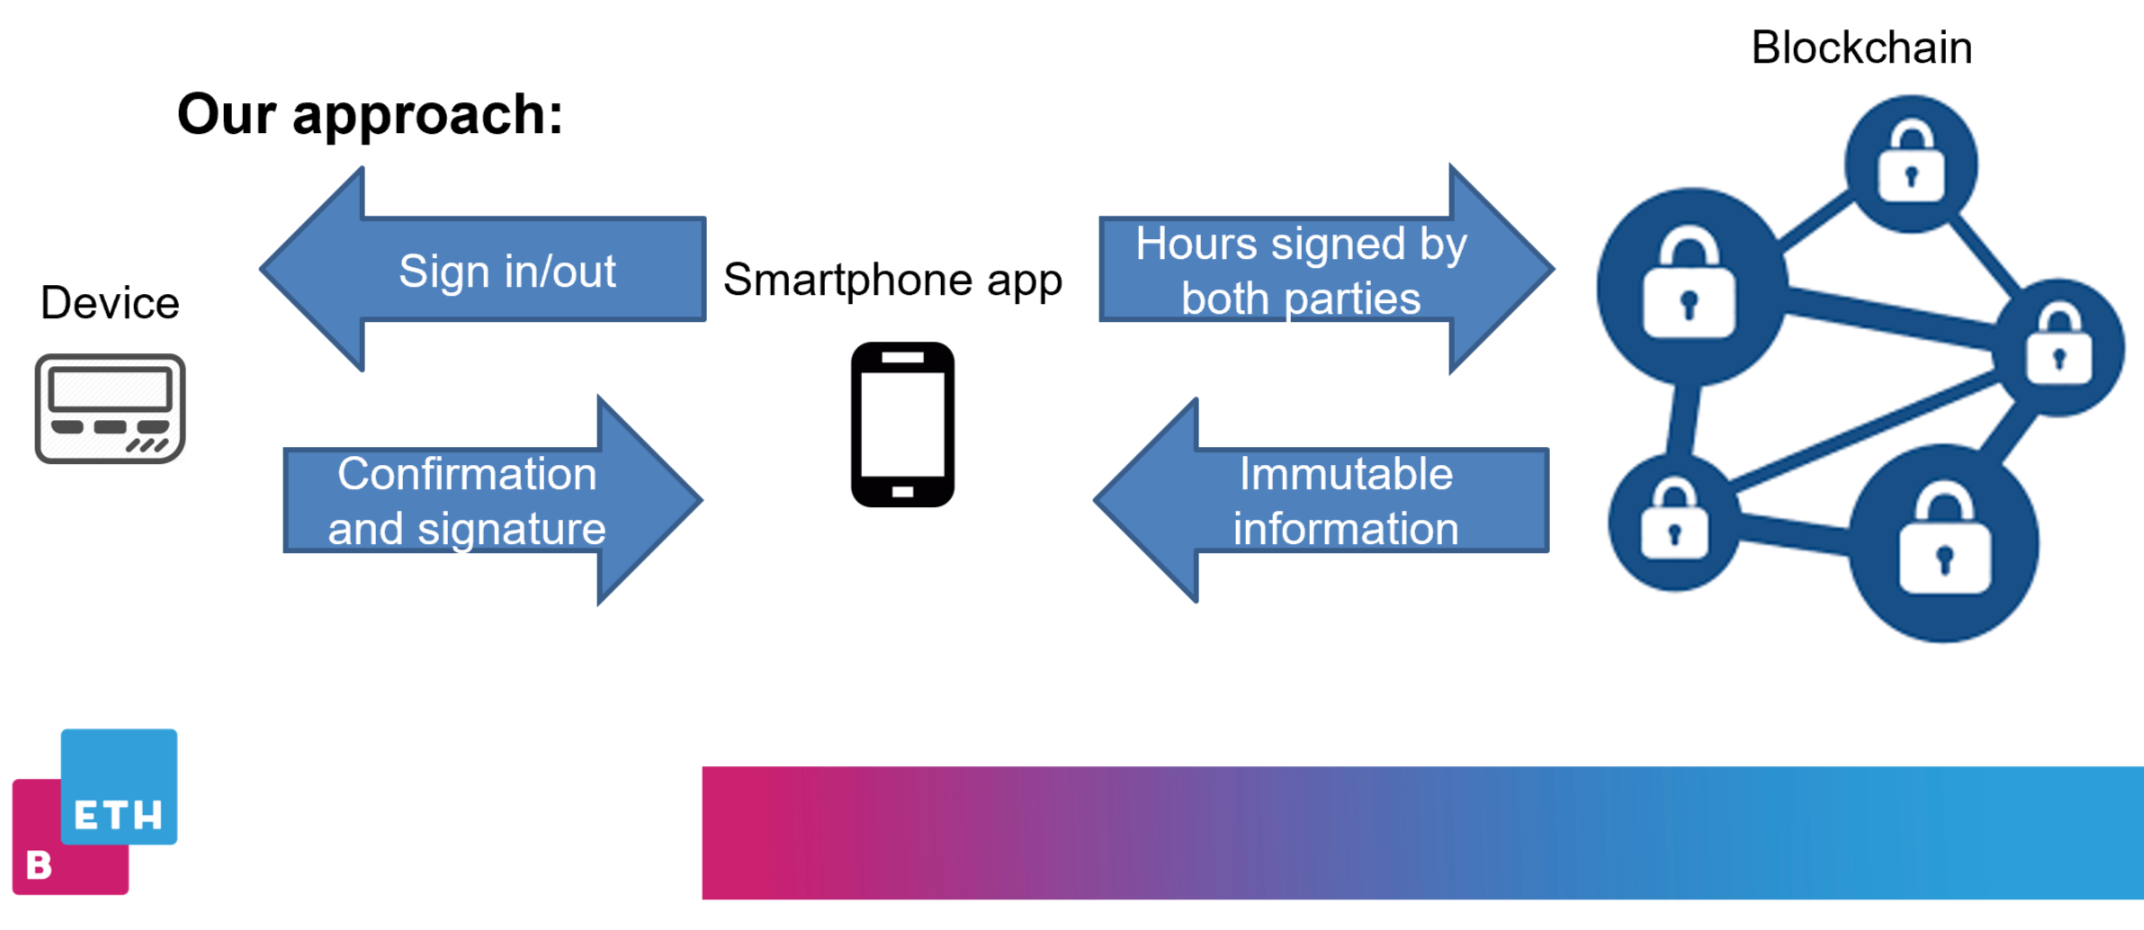
\includegraphics[width=12cm]{blockchain.png}
    \label{blockchain}
\end{figure}

As seen in Figure \ref{blockchain}, we divided our project into tho following three main parts:

\subsubsection{The Device}
We have built a device which is responsible for the time stamping. The caregiver logs on and off the service via interaction with the device. In addition, the KISS service receiver can indicate their satisfaction. We also invented a prototype badge to test our device.

\subsubsection{The Application}
We also designed an interface and developed a mobile application for the interaction between KISS-members. The application should be able to perform a new member registration. Furthermore, the clearly arranged interface should show the different kinds of offers which will be provided, just as in the KISS-catalogue.

\subsubsection{Backend and Contracts}
The third and last part of our project should realize the balance between privacy and transparency. On one hand, we want to keep activities secret from third parties in order to guard user data from exploitation. Therefore, we identify users only by their public key and we just log the time transactions onto the blockchain. On the other hand, the number of supplied hours should be accessible for everyone. This activity will be logged onto the blockchain and, by combining these guarantees with public key cryptography, we are able to provide authentication, non-repudiation and anonymity.
%\end{itemize}

\chapter{Design}

\section{Overview}
Our design builds on three main principles: sustainability, usability and trust. We create a sustainable solution by providing independence from third parties via the distributed ledger technology. The simplicity of our solution is rooted into the simple application interfaces provided for our KISS members and the intuitive hardware design for measuring time. Finally, we provide bidirectional trust between the donors and receivers by using public-key cryptography in combination with a distributed ledger and IoT devices.

Trust is a main concern both for our users and the KISS project backend. On one hand, any caregiver needs to be able to verify that his work hours have been correctly and durably registered. On the other hand, the project coordinators at KISS need to make sure that a caregiver has done the advertised work. We discuss this aspects in section \ref{backend}.

The next goal we defined was usability. We present an application that can be used by caregivers to both register user preferences regarding the assigned chores and to visualize time transactions in real-time. This is the first step towards reducing the paperwork needed in the association's pipeline by automation of the currently manual bookkeeping process of chores. The details regarding this application are discussed in section \ref{app}.

Finally, the interaction of the service receiver with administrative tasks should be both minimal and pleasant. We do this via an intuitive device that will be installed in the house of the service receiver. The purpose of this device is both providing trust in our application and allowing the service receivers to give feedback. We discuss the implementation of our device in section \ref{device}.


\section{Application}\label{app}

\subsection{Motivation}
Currently, the registration and time management of KISS is done manually which naturally comes with a lot of paperwork.

To cope with that, we have tried to set up a user interface that on the one hand handles registration as well as administration of the services the user wants to provide as well as time banking, and on the other hand is easy to use. Our first idea was to build a website as a prototype. However, since we also wanted to use a device which measures the time (as described in section \ref{device}) we decided to approach our goal by building an app which can interact with this devices via a smartphone.

\subsection{Approach}
We decided to use the \emph{React Native} framework for building the application. One reason is that React Native makes it easy to simultaneously develop for both \emph{Android} and \emph{iOS}. Another reason is that the applications can be built using only \emph{JavaScript} and \emph{React}.

%Our first goal was to get the framework running (just kidding)

Another objective was the ability of the application to present the services provided in a given period and the total amount of time the user has spent to help other people (comparable to \emph{online banking}). The user specifies a period over which he wants to have an overview of the completed ``transactions'' (services rendered). The time period and the user ID is then sent as a request to the backend, which returns the information about duration and nature of the activity as well as name of the person who was helped of every transaction that took place during this time.

In order to be able to interact with the device of the person who is being helped, we also wanted to integrate a wireless connection tool into the app which can connect the smartphone to the device (\emph{NFC}, \emph{Bluetooth}, \emph{WLAN}, etc.). This connection will be needed to authenticate the transaction described above: The application creates packets containing the information of the rendered service, but before putting it on the blockchain, it has to be authenticated by the device (this is explained in more detail in section \ref{crypto}).

Finally, we wanted to integrate the registration process into the app. Each user is assigned a unique ID, which is used to assign the transactions to the users and store them on the blockchain. This will allow the user to verify the transactions made and therefore create trust.

%The backend of the KISS project is still kept, but we replace the paper registration with an application. The application has a private-public key pair which can be used to sign a transaction together with the smart device.

\section{Backend and Contracts}\label{backend}

\subsection{Backend}
The backend component sits between the application and the blockchain. Let us motivate the need for a backend in a decentralized application.

Firstly, the KISS project already contains a classical backend service which function both for administrative purposes and derivative data analysis. We observe that the analytics functions together with parts of the administrative data(e.g. personal details, affiliations, chore preferences, etc.) are still well-suited for storage in a centralized manner both due to cost and privacy reasons.

Secondly, providing a gateway interface hides the user from the need of interacting directly with the blockchain. This may be desirable since transaction costs would have to be supported by the client, the client needs a wallet, etc. Furthermore, via the cryptographic primitives described in subsection \ref{crypto} we can achieve the exact same guarantees as if the client created a separate account.

\begin{figure}[h]
	\centering
	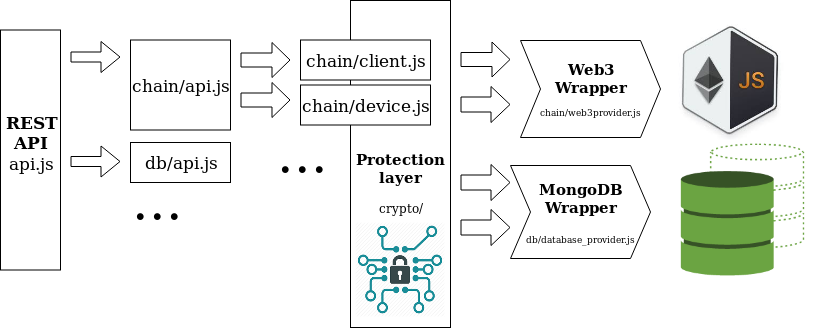
\includegraphics[width=0.8\textwidth]{backend.png}
	\caption{Backend components}
	\label{label:file_name}
\end{figure}

Now, let us discuss the design of the backend. By taking a glance at the picture above, one can observe that the data flows from left to right. This simple principle allows us to decouple services and add intermediate layer processing components, such as the protection layer that is realized via cryptographic primitives.

The mobile application can interact with the backend via a RESTful API. The calls made to this API are then redirected towards more specific APIs. The components get registered in the upper-level API, so that redirection can take place:
\begin{lstlisting}
export default class Api {
  register() {
    [...]

    new DBApi().register(this.server);
    new ChainApi().register(this.server);
  }
}
\end{lstlisting}

As an example, if a client wants to read the time balance from the blockchain, the request would be redirected to \texttt{chain/api.js}. The chain API would redirect the request to the particular file in which the handler sits, namely \texttt{chain/client.js}:

\begin{lstlisting}
export default class ChainClient extends Web3Provider {
  [...]
  handleBalance(conn, publicKey) {
    this.handleCall(conn, publicKey, 'getBalance', parseInt);
  }
}
\end{lstlisting}

As we will see in the cryptogrphic section, each client is identified by its public key. What happens in the code above is that we want to call a method on the blockchain, namely \texttt{getBalance}, and then parse the result we get and write it back to the supplied connection \texttt{conn}.

% looks odd otherwise
\newpage

\begin{lstlisting}
export default class Web3Provider {
  [...]
  handleCall(conn, publicKey, method, ret) {
    let theId = `0x${new Crypto().hash(publicKey).toUpperCase()}`;

    this.owner.then(owner => {
      this.contract.methods[method](theId).call().then(ret).then(x => {
          return { ans : x }
      }).then(x =>
        conn.send(x)
      );
    });
  }
}
\end{lstlisting}

The code above shows a part of the actual implementation of the \texttt{Web3 Wrapper} that facilitates communication with the \emph{Ethereum} blockchain. The purpose of the example was to notice a few characteristics of our backend design:
\begin{itemize}
    \item each class talks only to the lower and upper layers, making the design easily extensible
    \item each API component can filter a request if needed without damaging the message flow, making the design easy to secure
    \item the API request handlers form a tree, making the system easy to shard, hence scalable
    \item each upper-layer component can call methods on any low-level component (e.g. \emph{MongoDB}), making the low-level component transparent, hence easily replaceable
\end{itemize}

A major advantage of our approach is the opportunity for short-circuiting. That is, the backend can short-circuit the calls to reading the blockchain, using the \emph{MongoDB} component as a cache. The service is much faster than reading from blockchain, being able to provide the latest data. This means that the users have a much more interactive experience, being able to see their balance and latest transactions instantly.

The final point we make is that the backend design is easily adaptable to new features. As an example, we discuss how KISS could implement an opt-in service, that is, a user could make an \emph{Ethereum} account and interact with the blockchain directly. Since each service is self contained, we only need to create a thread on the server reads the most recent calls on the contract and updates the information kept in the backend. This can be done only by using the components \texttt{Web3 Wrapper} and \texttt{MongoDB Wrapper}.

\subsection{Cryptography}\label{crypto}
The cryptographic part is a central component of our service. The main goal of it is providing bidirectional trust between the server and the client by using the device. The workflow of the process uses public-key cryptography together with the blockchain's guarantees and is described in the figure below.

\begin{figure}[h]
	\centering
	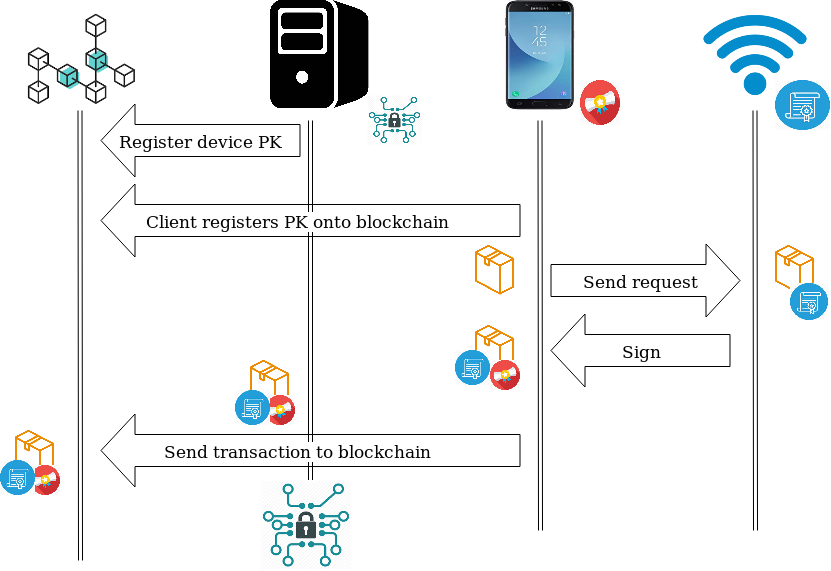
\includegraphics[width=0.9\textwidth]{crypto.png}
	\caption{Cryptographic workflow}
	\label{label:file_name}
\end{figure}

In the first step of the process, the device is registered onto the blockchain before being given to the service receiver. Now, each KISS member needs to register its public key with the backend, so that the contracts only keeps information relevant to the KISS project. These steps are represented by the first two arrows in the diagram above. Devices and clients are identified by a public key(denoted PK on the diragram) from a public-private key pair. Note that the key pair is generated at the respective client/device, hence the server does not know any of the private keys.

In the next step, the client (that is the Android application of the user) creates a packet containing its public key to send to the device for signing. The communication path can be any wireless channel. When the device receives the packet, it will wait until a button is pressed for finishing the session. At this point in time, the volunteering session has finished and the packet is augmented with the amount of time and a counter. The augmented packet(referred to as packet from now on) will be signed by the device and sent back to the mobile application. This is represented by the third arrow in the diagram.

At this point, the client has all the necessary information for publishing the transaction onto the blockchain. He also has the guarantee that the device did the correct job since its own public key is contained in the packet. Finally, to publish onto the blockchain the client will sign the packet as well and send it to the blockchain either thorough the backend(current implementation) or directly. The final data stored onto the blockchain is:
\begin{lstlisting}
(clientPK, devicePK, amount, clientSignature, deviceSignature, counter)
\end{lstlisting}

The verification of the transaction can be done by anyone, and to reduce the data kept onto the blockchain the backend will verify the transaction before publishing. We mention that we also have a variant of the smart contract that verifies the transaction, but the initial contract(and the one we use now in the implementation) allows anyone to store a transaction onto the blockchain. However, all the needed data is onto the blockchain, hence all transactions can be verified by any 3rd party.


\subsubsection*{Guarantees}

The protocol we described provides several guarantees:
\begin{itemize}
    \item privacy - each client is identified by its public key, hence only KISS knows client's name
    \item authentication - only the client (the app) can claim the tokens since only the client knows the private key
    \item non-repudiation - only data signed by the device provides the integrity guarantee, fact verifiable by anyone
    \item freshness - time transactions can't be replayed since the device generates a new counter value for each transaction
    \item immutability - from the blockchain guarantees
    \item tamper-evident - from the blockchain guarantees and signatures
\end{itemize}

\subsubsection*{Possible attacks}

We discuss a series of attacks our algorithm is resilient against:
\begin{itemize}
    \item client replays transaction: not possible since the device is tamperproof and transactions are fresh
    \item server replays transaction: not possible since server does not have a device signature for the next counter
    \item server uses smart device to replay transaction: not possible since server does not have the client signature for the next counter
    \item rollback attacks: not possible since the counter only increases on the blockchain
    \item server excludes transaction: this is possible, but detectable from by the log of transactions stored onto the blockchain
\end{itemize}

However, our protocol is not protected against more powerful attackers:
\begin{itemize}
    \item attacker has access to device, user and backend: a possible mitigation is employees not being able to make an account
    \item attacker that can tamper with device: a possible mitigation is making the device tamper evident
\end{itemize}

\subsection{Blockchain}
%\textbf{TODO[Johannes]}
The blockchain part of our application is used as a tracker of \emph{TimeTokens}. It should store the amount of \emph{TimeTokens} for each person participating and provide a list
of transactions that contain a proof mechanism such that both donor and receiver have accepted and validated this transaction.
Additionally we want to store as less data as possible on it, since space on the blockchain is limited and we don't want to store too much data publicly because much of the data is sensitive and could be easily abused for criminal purposes.
An other criteria is that organisations or even people directly could participate in the system and validate all the transactions without the help of KISS or any other organisations such that we build trust between all parties.

 To solve these requirements we built a smart contract that contains the following data structures:
\begin{itemize}
\item A mapping from an address to a client object. The client object contains the TimeToken balance of the client and the counter used to validate that the same transaction is not made multiple times.
Donors and receiver of services are clients in this data structure.

\item A list of transaction objects.
A transaction object is equal to a service a donor provided to a receiver and contains the addresses of the donor and the receiver as well as the amount of time, the counter we mentioned above and a signature from both the donor and the receiver.
The signatures are made over a string that contains the donor of the service(his public key), the amount of time he spent and the counter.
\end{itemize}
The functionalities the contract has to provide are, the normal functions an ERC-20 token should provide such that something can be done with the token in the future, registration of clients, a function that adds and automatically validates transactions and normal getter functions that let users read the stored data.

The signatures now can be used as a proof mechanism such that everybody can always check whether a transaction is valid.
An insurance company or other parties interested in this system for can easily verify that that both parties agreed that a service was done.

What the blockchain doesn't do is provide names or other identification for donors or receivers of services.
In my opinion this wouldn't be a good idea since this data could easily be abused.

\section{Device}\label{device}
%\textbf{TODO[Yves, Betim]}
%\\
\subsection{Purpose}
When it was clear which challenge we were into, we talked to the staff of KISS. They wanted an easy time banking system where they could track and measure time easily. It had to be simple to use for service receivers with no knowledge of smartphones etc. so the idea of a «easy to use device» came up. We decided that this device should measure the time and include a feature for the service receiver to give a feedback for the received service. To keep it simple, we wanted a badge system where the caregiver can badge in to start the time measurement. After the caregiver provided the service, he just needs to badge out again and the service receiver can press a button with a smiley face according to the quality of the service. This data $-$ time and feedback $-$ and a signature should be sent to the smartphone of the caregiver and from there onto the blockchain.

\subsection{Build}



After we had an idea what the KISS staff wanted, we came together and decided what features our device needs to fulfill these requirements. So building the device consisted of 3 challenges: First, we had to make the check in/check out function, then include a feedback option and finally get the data on the PC(later smartphone). We decided to use the following materials: an Arduino nano, 3 Push Buttons, one LED, Bluetooth module, \emph{NFC} reader, \emph{NFC} chip and some resistors.


Already in the first challenge we faced a problem: There were no \emph{NFC} chips nor \emph{NFC} readers so we decided to simulate this check in / check out procedure with a magnet and a hall sensor. Hall sensors recognize a near magnetic field so when we held the magnet near the device the sensor sends a signal to the micro controller.

The Push buttons were pretty easy to realize. We could attach them directly to the Arduino nano so whenever they get pushed, they send a signal directly to the micro controller. The LED was also really easy to implement. In series with a resistor we could attach it to the Arduino nano.

\begin{wrapfigure}{R}{.\textwidth}
	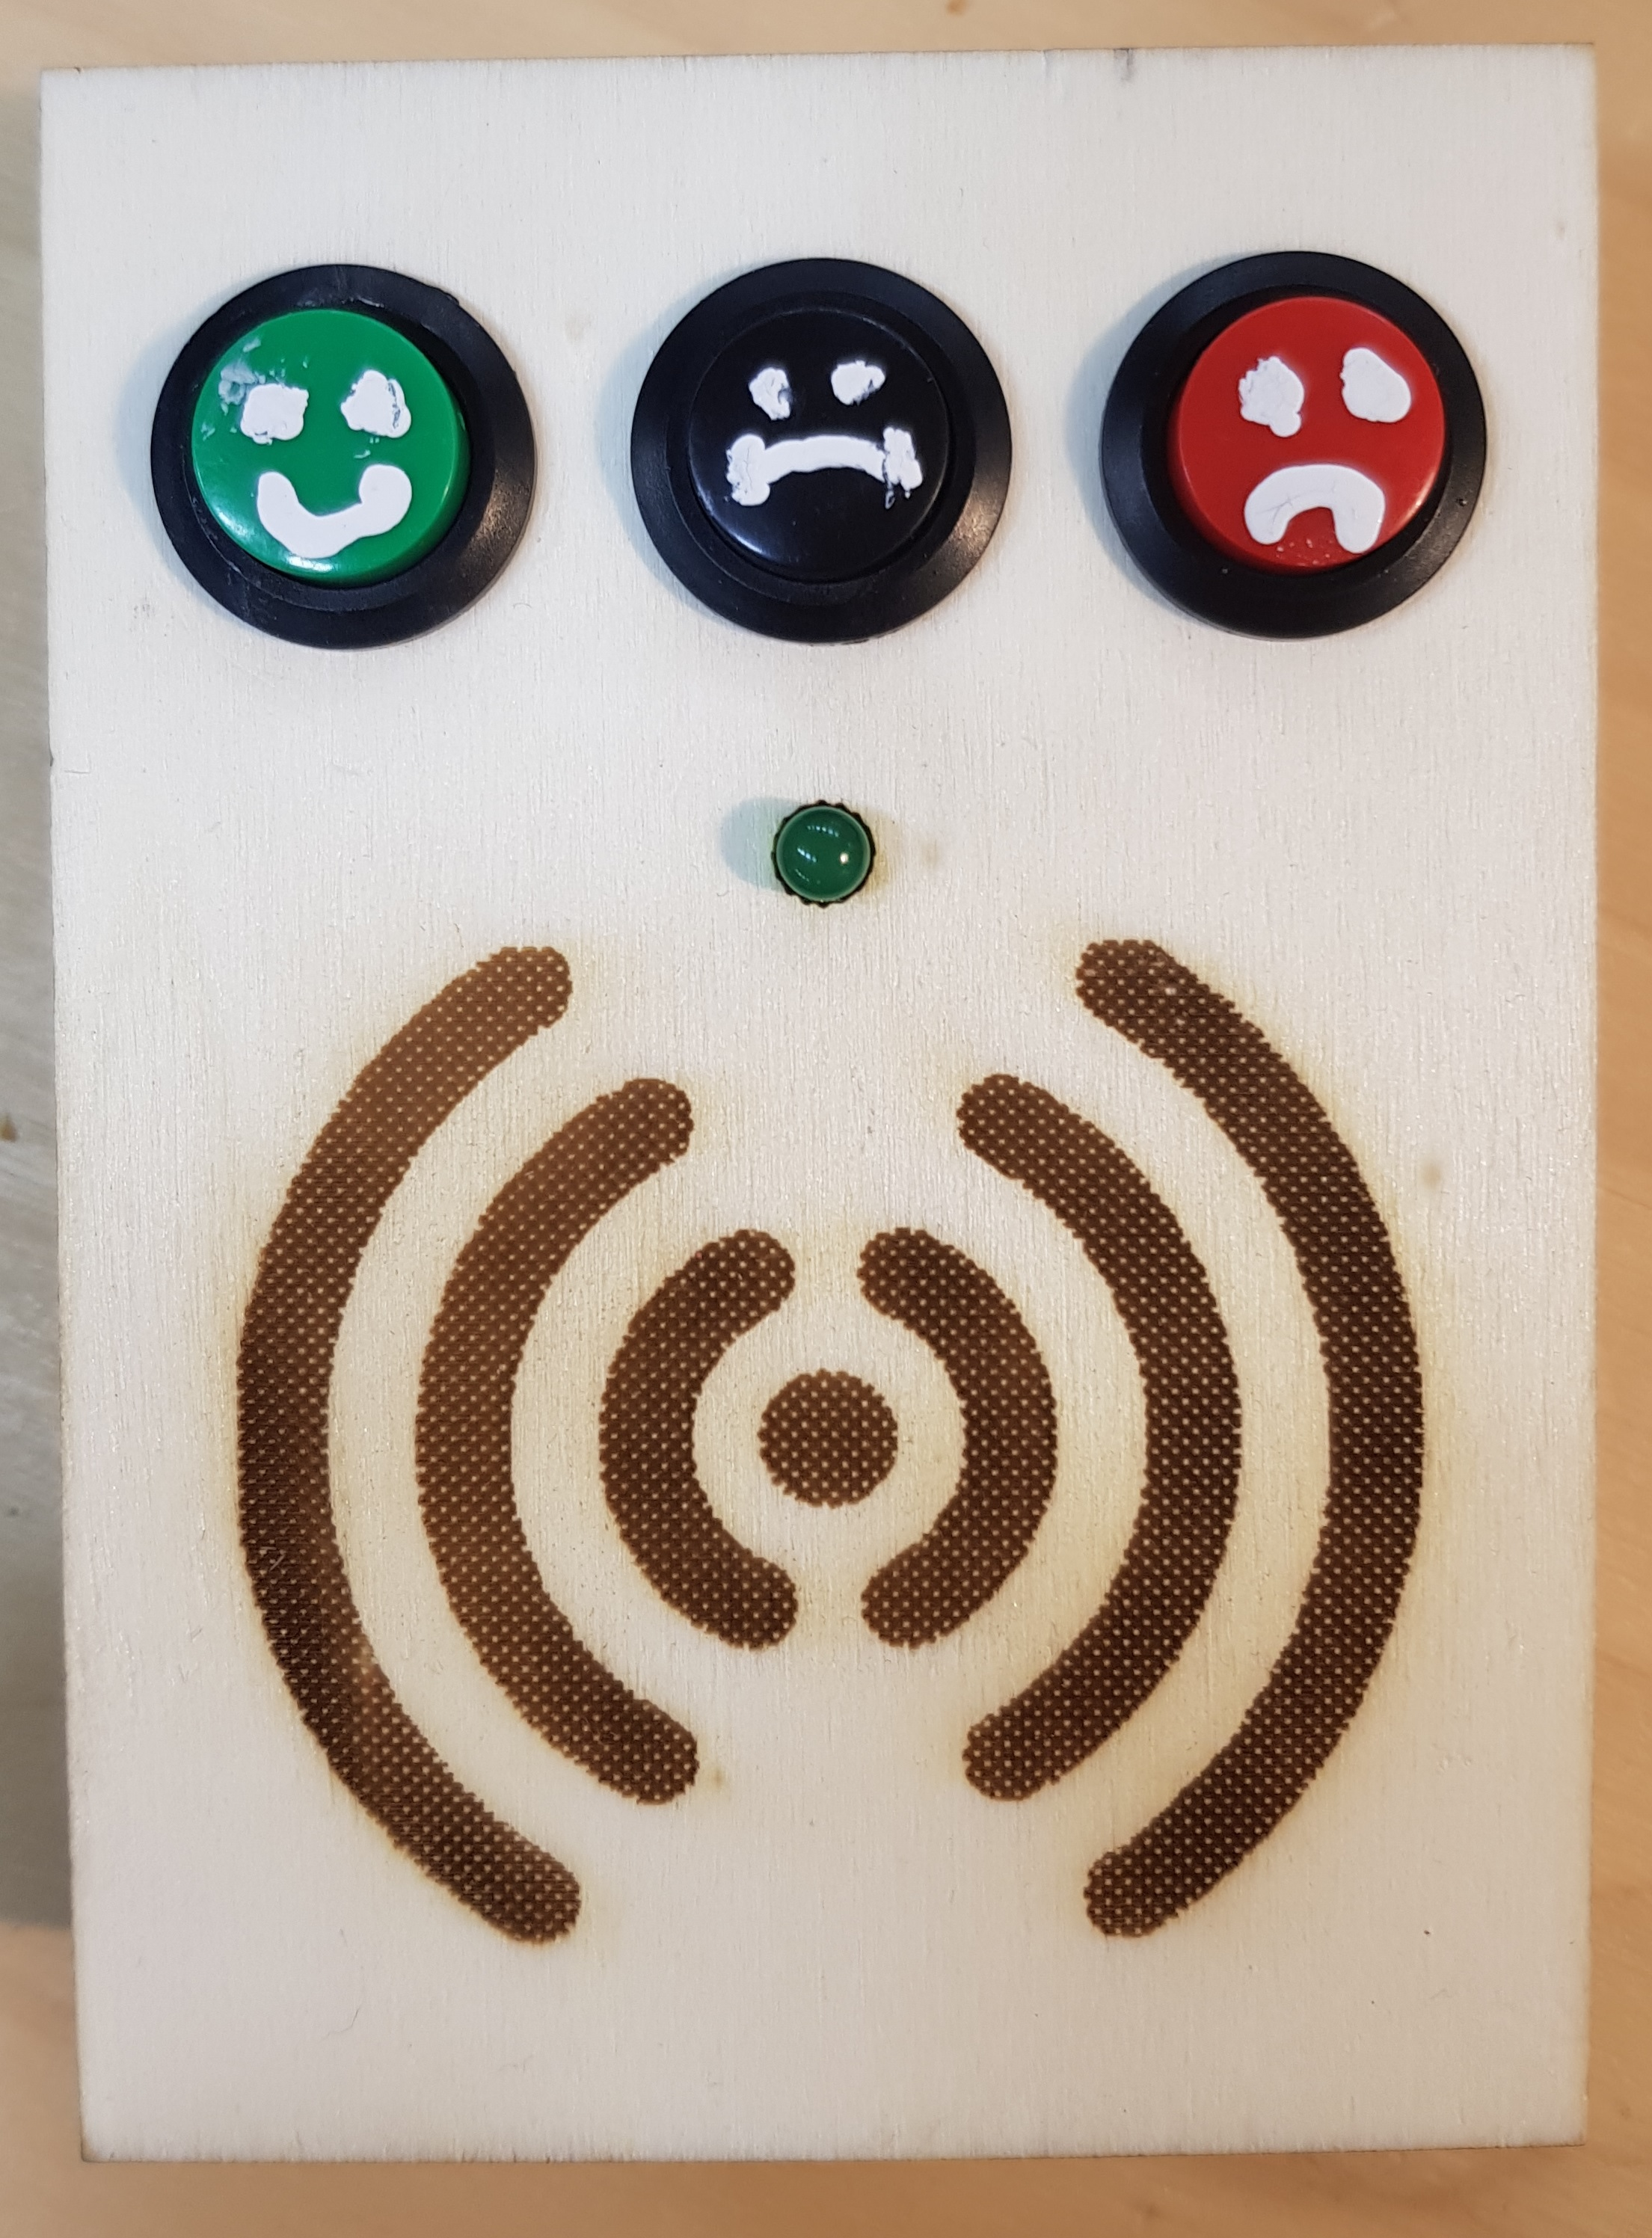
\includegraphics[height=4cm]{devicelatex.jpg}
    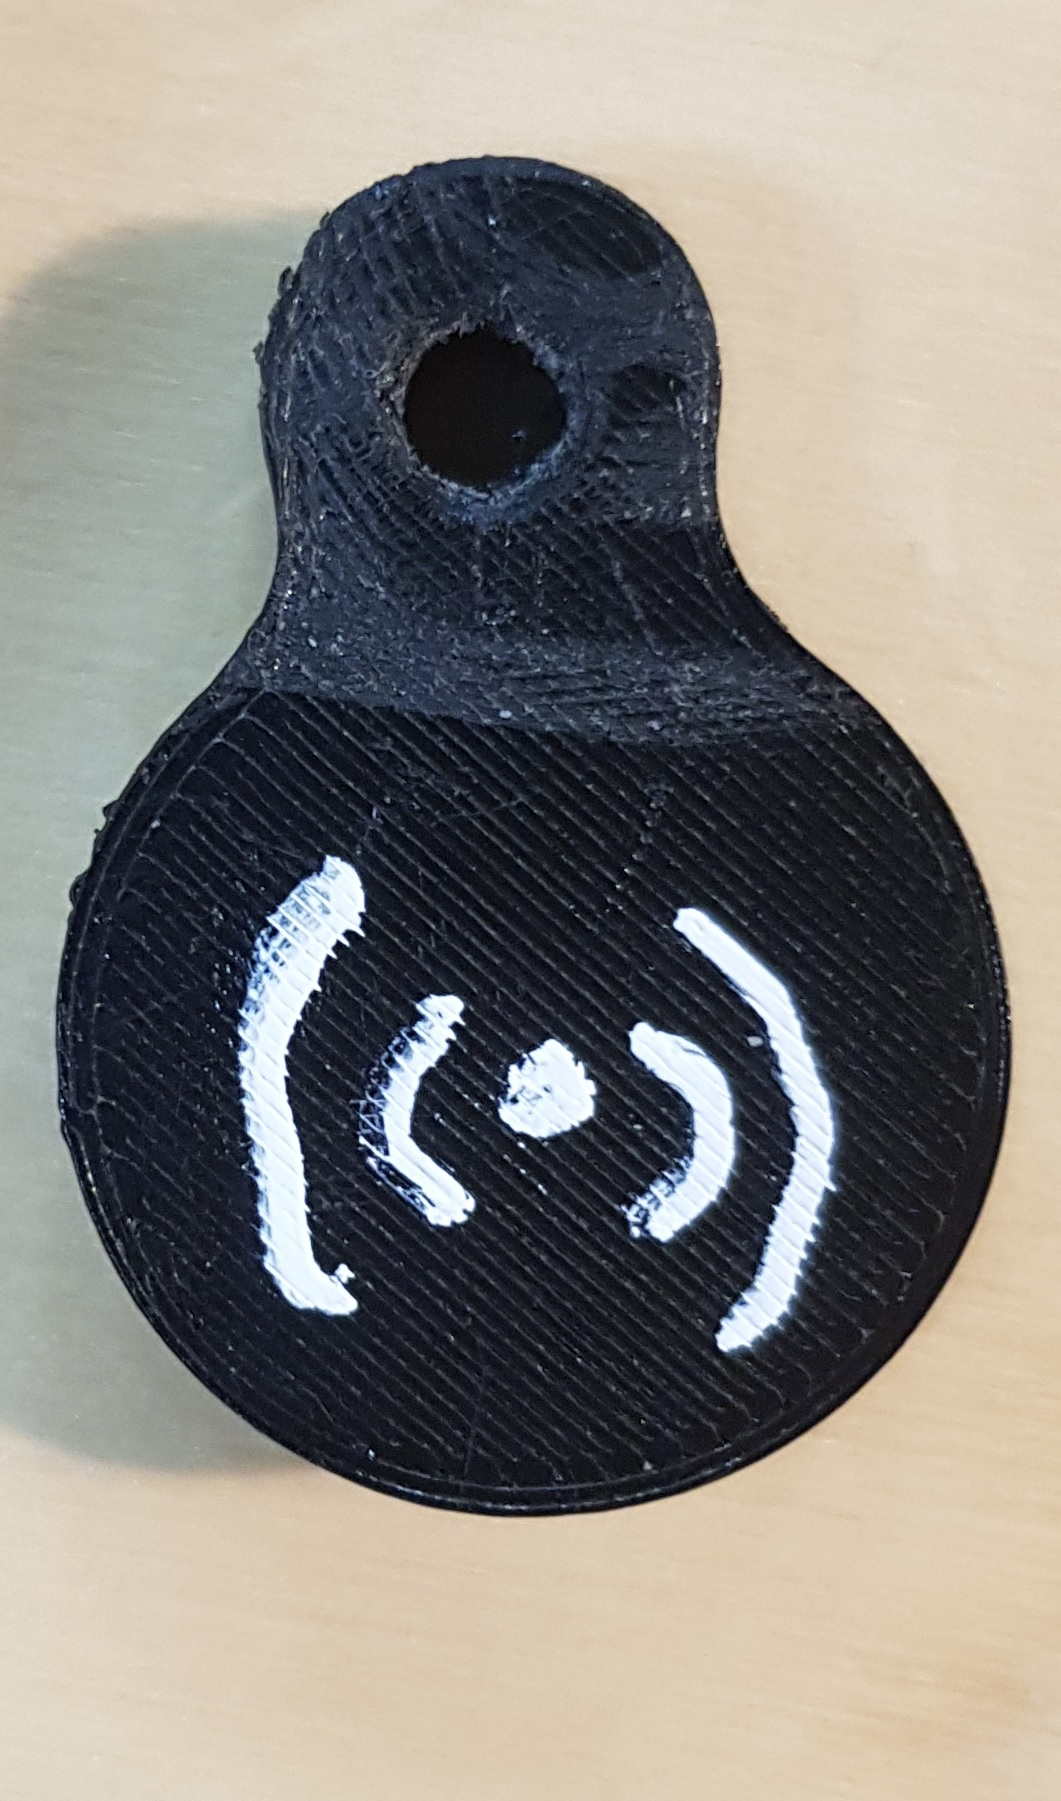
\includegraphics[height=4cm]{badgelatex.jpg}
	\caption{The device on the left and the small badge on the right}
	\label{label:manometer}
\end{wrapfigure}

The \emph{Bluetooth} module was another challenge we faced. It did not work properly, no matter what we tried. Normally you turn these modules on and they should be able to connect to devices such as smartphones but the modules we got were all broken or just very unintuitiv to use. We wasted almost a day with trying to get it to work but we had no luck. Later after the BETH challenge we tried to connect a different \emph{Bluetooth} module and it worked on the first try. However, since the \emph{Bluetooth} connectivity seemed not to be working we decided to use a USB cable connection to transmit the data to the PC.

As soon as it was more or less obvious how the internal of our device should look like, some members of our team got to designing the case for our device. We designed it in Siemens NX and manufactured it with laser cutter out of 4mm Plywood. The badge was simply a magnet in a 3d printed case.

Writing the code was not a very big problem. The Code for the micro controller was written in the Arduino IDE. The received data from the Arduino nano was processed with the program «Processing 3» in which we could display the data(name of the service receiver, time passed and feedback) in a graphical user interface.



\chapter{Evaluation}

\section{Discussion}

% \textbf{TODO[Philip]}: about advantages \& drawbacks, see slides 3, 4 @ BETHerCareSubmissionSlides

\subsection{Disruption Potential}

In the following section, let me discuss and evaluate the disruption potential of the KISS idea implemented in our way as described earlier. In the economic sense, a disruptive idea is generally known as an innovation that creates a new market by applying new techniques or pursuing a novel design philosophy which then lead to the disruptive idea effortlessly outperforming the conventional approach. In recent times, leveraging new technologies arising from computer science, especially the internet, has often led to such disruptive businesses.

The blockchain, or more generally distributed ledger technology, is yet another technological invention that seems to bear great potential for giving rise to many disruptive ideas in all kinds of fields. Let me now come to the reason why this is also true for the field of health care and especially the idea of time banking.

If we think about what characteristics would constitute a well designed old-age provision system, two of the most important and somewhat related objectives that immediately come up are trustworthiness and independence from a central controlling entity. When trying to solve these problems using technology these days, a distributed ledger seems to be almost the obvious choice, since its very purpose lies in enabling a trusted way of decentralizing systems and still being able to achieve consensus among the parties involved.

Old-age provision can basically be seen as a agreement among society that younger people are obligated to support elderly people who rely on help. When the younger ones are old themselves it's up to them to profit from the support of the next generation. As we see this basic description does not include any controlling third party. Hence in an ideal implementation of such a system, it would be natural not to introduce any third party as well. Of course up to now, some central party has been necessary to ensure that caregivers are contributing their part to the agreement and not acting selfishly. Our approach using the blockchain as a tool providing trust has the potential to truly turn old-age provision into a contract just between generations as it is naturally meant to be.

The KISS idea implemented using blockchain technology thus has indeed high disruption potential, although this potential is not primarily in the economic sense as first described but rather disruption in terms of democratizing society by removing its need to rely on a third party to enforce its internal agreements.


\subsection{Negative Aspects and Open Challenges}
\begin{itemize}
    \item The Source of trust is guaranteed but not easily understandable by the average person without a background in technology (especially hard for elderly people).
    \item Trust is only ensured on a high level, making sure that what gets recorded on the blockchain is what actually happens in the real world is a different story.
    \item In the current state of distributed ledger technology, transaction costs are relatively high. However this might improve with time since it's still a young, but actively researched, technology and could mature in the near future.
\end{itemize}


\section{Current State}

\subsection{The App}

\begin{figure}[!ht]
	\centering
	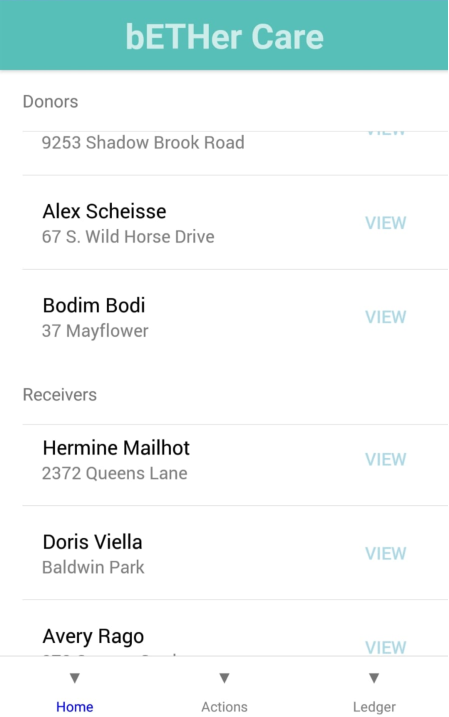
\includegraphics[width=0.3\textwidth]{App_Home.pdf}
	\quad
	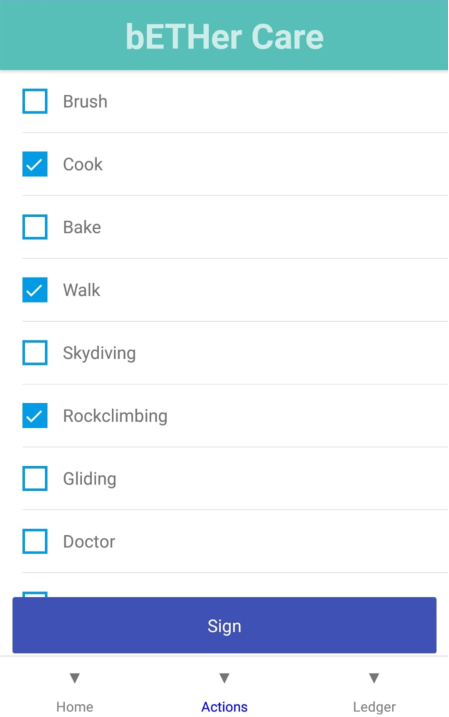
\includegraphics[width=0.3\textwidth]{App_Actions.pdf}
	\quad
	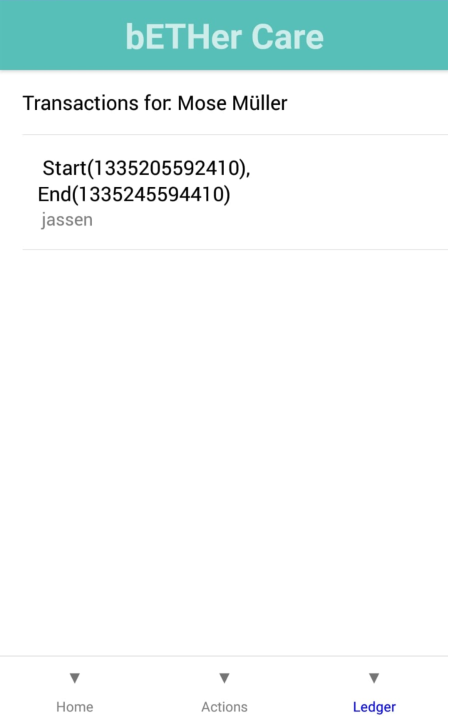
\includegraphics[width=0.3\textwidth]{App_Ledger.pdf}
	\caption{The graphical user interface of the application. The first menu tab lists all donors and receivers, the second tab enables to specify the services one wants to provide. The last tab lists all the rendered activities (duration and kind of activity).}
	\label{Application}
\end{figure}
%\textbf{TODO[Mose]} about app \\

The application has a graphical user interface which can be seen in Figure \ref{Application}. Different features are organized via a simple menu at the bottom. The user can select and save activities he or she wants to provide (menu item ``Actions''). This data is saved on the mobile phone and not connected to the database yet.

In addition, we have implemented a listing of caregivers and service receivers. These are displayed with the name as well as address (menu item ``Home'') and retrieved from the backend via an API request.

We also implemented a view of the services one has provided in a given period. They can be accessed via the menu item ``Ledger''. We could further improve this by adding a form where the user can specify the period of time for which he or she wants to retrieve the information and in addition, display the total amount of time he or she has spent helping others.

In the attempt to connect the caregiver's smartphone to the service receiver's device, we implemented a \emph{Bluetooth} interface into the app. However, since the \emph{Bluetooth} module did not work properly on the device, we stopped working on this feature and later removed it from the app.

Unfortunately, realizing that we would not have enough time to get it working properly, we did not work on the registration part.

%What we tried to implement, was that People who want to work with the KISS network could simply track their time on the blockchain with the help of a simple to use device which signs each transaction for the receivers of the work. In the future the app should directly interact with the blockchain instead of the backend API. This was not possible as of today because of the transaction costs of the blockchain. \\We got the communication between the app and the backend api working.


\subsection{The Backend}

%\textbf{TODO[Johannes]} about backend \\
For the backend, we built a first, working smart contract that provides some of the functionality we wanted to implement.
What is still missing, is the automated validation of transactions signatures and the ERC-20 token functionalities.
At the moment the contract is built such that we need an owner who does all the administrative part like adding transactions and users.
In the future it should obviously be possible for each client to register and add transactions himself.
Generally this first version of the contract can still be much improved.

Additionally we provided a version two of the contract which improves some of the faulty design we made in the first contract.
We also tried to add the automatic validation of the transactions which we unfortunately couldn't finish in time.

Some parts of the interaction between the backend and the blockchain were implemented but haven't been tested in the end because we focused more on reworking the smart contract since the faulty design provided many problems to the interaction.

A large part of the cryptographic operations have been implemented into the backend API. Even though not all the operations have been implemented in the backend API, we provide fully-functional cryptographic prototypes in the \texttt{server/crypto} folder. The same primitives have been deployed onto the Android application for signing and interacting with the device.


\subsection{The Device}

%\textbf{TODO[Betim]} about device  \\
The device has been designed to be as simple as possible, so that people with no technical knowledge can use it without being reliant on others. At the moment it is possible to get the information out of the device to the PC with a USB-port-connection. The idea was to get the information to a smart phone via \emph{Bluetooth}, so that the service receiver don't need to do anything. The problem we had was, that we hadn't a \emph{Bluetooth} that worked with our setup. We had to choose another way to show our prototype so we put a sensor that recognize magnetic field. As soon as a magnet goes through the magnetic field, the sensor send a signal to the control module and the time starts respectively the time ends counting.

The device is meant to be for checking in or out the helper and to measure the time he spend and for giving them an evaluation. The evaluations had also to be as simple as possible, so we decided to design a device with tree buttons. The green button means that the care was good, so they would like to meet them again .The black one means that the care was okay (neutral opinion) and the red one means that the care was bad, so they don't necessarily want to meet them again.

Currently the device doesn't work the way we wanted because of the limited hardware we could use, but the principle idea works. It's possible to check in and to check out and also to measure the time they spend together. The evaluation buttons work too. The only thing that does not work at the moment is the connection with the smartphone.


\section{Issues}

\subsection{Mobile Application}
%\textbf{TODO[Philip]} about app \\
At the first day of the hackathon, we decided to use the \emph{React Native} framework for building mobile apps using \emph{JavaScript} and \emph{React}. This seemed to be a reasonable decision, since it not only supports cross-platform compatibility (\emph{iOS} and \emph{Android}), but it would also allow us to use \emph{JavaScript} as the primary language throughout the whole project. Also \emph{React Native} should make the design and implementation of a simple user interface for the app easier, because of the \emph{HTML}-like declarative language and the large amount of predefined UI components available.

In hindsight however, going for a native \emph{Android} app might have been the better choice because none of us had worked with \emph{React Native} before. Setting it up for the first time was quite a mess and took us much longer than we though. Fortunately, we still managed to create the most important parts of the interface and could eventually even send and receive content from the backend and have it show up in the app.

\subsection{Backend}
%\textbf{TODO[Johannes]} about backend \\
The main issues we had in the backend as well as anywhere in the project was the lack of experience we had in the group.
Nobody ever worked with one of the technologies we used in this project so we had to use much of our time to get to know the concepts behind the technologies such as the blockchain and smart contracts.
Because of this lack of knowledge we had to discard many ideas or concepts we had because they were fundamentally wrong or just to time-consuming or complex to implement.
This also reflects in our code.
Most of the code we wrote was very messy because we tried to do something but then realized somewhere in the middle or even after we finished something, that it's not the right way to do it.

A good example for this would be the smart contract. The differences between the first and the second version are already huge and
we could certainly still improve a lot on the second one.

Most trouble came from working with the \texttt{web3.js} library and from the interaction between backend and frontend.
Since we had almost no blockchain experience in the group, we had trouble to grasp the concepts behind it, how the accounts, tokens, currencies, etc. really work and how we could build the interaction between our application and the blockchain.
The issues we had with the interaction between the frontend and backend could be solved in the end but were still very time consuming for us.

\subsection{Device}
%\textbf{TODO[Betim]} about device\\
As it was mentioned before we had a problem with setting the device up with a \emph{Bluetooth} or wireless. We bought a \emph{Bluetooth} in project house, but for some reasons we couldn't connect it with Arduino no matter what we tried. So we tried with wireless and we had the same problem. The \emph{Bluetooth} and wireless we had, were unknown, so we couldn't find anything in internet that could help us solving the problem. We also asked the people in student project house for some help but unfortunately they couldn't help us at all. The result was that we decided to evade this problem and did with magnetic field and a magnet.

To get the data to the smart phone was also a problem. We didn't waste a lot of time at this problem, because in the future it's not meant to get the data from the device in a computer and then from the computer to a smartphone. The device should be able to send the data directly to the smart phone via \emph{Bluetooth} or wireless.
The other problems we had were mostly not so big and we could solve them easily.


% looks odd otherwise
\newpage

\section{Future Improvements}
In summary one can say that many parts of the intended system's skeleton could be built, like the backend API connecting to the blockchain and providing data to the application that also works and features a basic interface for viewing a time banking account and one's recently provided services. Additionally we managed to build a easy-to-use device that can be placed in an service receiver's home and is used to verify that services were actually provided. What is missing in this basic skeleton is the connection of app and the just described device via \emph{Bluetooth} or \emph{NFC} as well as some of the cryptographic functionality and the whole system could never be tested on an actual blockchain. Adding those parts would make it a complete proof of concept.

Apart from that, this is of course just the basic structure and for an actual deployable system, many more functions would have to be implemented, for example a registration form in the app plus corresponding functionality on the API provided by the backend.


\chapter{Conclusion}

In summary, one may conclude that the general idea of using the blockchain as the underlying technology to base a modern old-age provisions system on seems promising. Eliminating the need to rely on a trusted third party to control the whole process and manage the ``time bank'' blends well into the concept of old-age provisions as a contract between generations. Detaching agreements within society from a powerful, controlling unit would definitely make the world a \emph{bETHer} place.

It does not come as a surprise that turning these abstract ideas into a working prototype during a hackathon while still learning how the technology actually works is not an easy thing to do. As described earlier, we have been faced with all kinds of issues when implementing the app and the backend with its cryptographic parts and the interaction with the blockchain, as well as when building the physical device as an easy-to-use interface. Besides that, we still achieved some solid results, since we were able to build a working subset of the described system including communication between our app and the backend. And if nothing else, we all learned a lot from this intense week, because almost none of us had ever worked with any of the tools we have been using before.

To sum it all up, what starts with a promising idea in theory, as always turns out to be harder than expected to implement in practice. However, this project did result in a basic working skeleton for the described system and can, in our eyes, be seen as a solid basis for future work and improvements.




%\newpage
%\chapter*{References}

%[2]John W. Eaton, David Bateman, Sren Hauberg, Rik Wehbring (2015). GNU
%Octave version 4.0.0 manual: a high-level interactive language for numer-
%ical computations. Available: http://www.gnu.org/software/octave/doc/
%interpreter/.

\end{document}

%-------------------------------------------------------------------------------
% SNIPPETS
%-------------------------------------------------------------------------------

%\begin{figure}[!ht]
%	\centering
%	\includegraphics[width=0.8\textwidth]{file_name}
%	\caption{}
%	\centering
%	\label{label:file_name}
%\end{figure}

%\begin{figure}[!ht]
%	\centering
%	\includegraphics[width=0.8\textwidth]{graph}
%	\caption{Blood pressure ranges and associated level of hypertension (American Heart Association, 2013).}
%	\centering
%	\label{label:graph}
%\end{figure}

%\begin{wrapfigure}{r}{0.30\textwidth}
%	\vspace{-40pt}
%	\begin{center}
%		\includegraphics[width=0.29\textwidth]{file_name}
%	\end{center}
%	\vspace{-20pt}
%	\caption{}
%	\label{label:file_name}
%\end{wrapfigure}

%\begin{wrapfigure}{r}{0.45\textwidth}
%	\begin{center}
%		\includegraphics[width=0.29\textwidth]{manometer}
%	\end{center}
%	\caption{Aneroid sphygmomanometer with stethoscope (Medicalexpo, 2012).}
%	\label{label:manometer}
%\end{wrapfigure}

%\begin{table}[!ht]\footnotesize
%	\centering
%	\begin{tabular}{cccccc}
%	\toprule
%	\multicolumn{2}{c} {Pearson's correlation test} & \multicolumn{4}{c} {Independent t-test} \\
%	\midrule
%	\multicolumn{2}{c} {Gender} & \multicolumn{2}{c} {Activity level} & \multicolumn{2}{c} {Gender} \\
%	\midrule
%	Males & Females & 1st level & 6th level & Males & Females \\
%	\midrule
%	\multicolumn{2}{c} {BMI vs. SP} & \multicolumn{2}{c} {Systolic pressure} & \multicolumn{2}{c} {Systolic Pressure} \\
%	\multicolumn{2}{c} {BMI vs. DP} & \multicolumn{2}{c} {Diastolic pressure} & \multicolumn{2}{c} {Diastolic pressure} \\
%	\multicolumn{2}{c} {BMI vs. MAP} & \multicolumn{2}{c} {MAP} & \multicolumn{2}{c} {MAP} \\
%	\multicolumn{2}{c} {W:H ratio vs. SP} & \multicolumn{2}{c} {BMI} & \multicolumn{2}{c} {BMI} \\
%	\multicolumn{2}{c} {W:H ratio vs. DP} & \multicolumn{2}{c} {W:H ratio} & \multicolumn{2}{c} {W:H ratio} \\
%	\multicolumn{2}{c} {W:H ratio vs. MAP} & \multicolumn{2}{c} {\% Body fat} & \multicolumn{2}{c} {\% Body fat} \\
%	\multicolumn{2}{c} {} & \multicolumn{2}{c} {Height} & \multicolumn{2}{c} {Height} \\
%	\multicolumn{2}{c} {} & \multicolumn{2}{c} {Weight} & \multicolumn{2}{c} {Weight} \\
%	\multicolumn{2}{c} {} & \multicolumn{2}{c} {Heart rate} & \multicolumn{2}{c} {Heart rate} \\
%	\bottomrule
%	\end{tabular}
%	\caption{Parameters that were analysed and related statistical test performed for current study. BMI - body mass index; SP - systolic pressure; DP - diastolic pressure; MAP - mean arterial pressure; W:H ratio - waist to hip ratio.}
%	\label{label:tests}
%\end{table}%\documentclass{article}
